\section{GitHub Repository}\label{sec:github}
 The source code for this report and every code inhere mentioned can be found in the following GitHub repository: \href{https://github.com/CarlosPuga14/MetodosNumericos_2024S1}{CarlosPuga14/MetodosNumericos\_2024S1}.

\section{Main Function Code} \label{sec:mainFunction}
The main function code is shown in Listing \ref{code:main}.
\begin{lstlisting}[language=Python, caption={Main function.}, label={code:main}]
def Main()->None:
    decomposition = "LDLt"
    pivoting = True
    diagonal = False

    output_file = f"{decomposition}" 
    output_file += f"{'_Pivoting' if pivoting else ''}"
    output_file += f"{'_Diagonal' if diagonal else ''}"
    output_file += ".txt"

    matrix = # given Matrix  
    
    full_matrix = FullMatrix(matrix, pivoting, diagonal, decomposition)

    full_matrix.PrintMathematica(True)
 
    full_matrix.Decompose()
    full_matrix.FindInverse()
    full_matrix.Print(output_file)

    full_matrix.CalcMemoryUsage()

    vec = np.random.rand(full_matrix.A.shape[0])
    sparse_matrix = SparseMatrix()
    sparse_matrix.ParseFullMatrix(full_matrix.A)

    sparse_matrix.CalcMemoryUsage()

    a = sparse_matrix.Multiply(vec)

    b = np.dot(full_matrix.A, vec)

    print(np.allclose(a, b))

    sparse_matrix.EvaluateSparsity()
\end{lstlisting}
Lines 2 to 13 set the input data for the FullMatrix object. Line 15 turns on the Mathematica way of printing output. Lines 17 to 19 decompose, invert, and print the output for the given matrix decomposition. Line 21 calculates the memory usage, used later to compare with the sparse matrix. 

Line 23 creates a vector of random numbers to test the multiplication of the sparse matrix. Lines 24 to 27 create the SparseMatrix object, parse the full matrix, and calculate the memory usage. Line 29 calculates the multiplication of the sparse matrix by the vector, while line 31 does the same for the full matrix. Line 33 compares the results. 


\section{Permutation Matrices}\label{sec:PermutationMatrices}
Figures \ref{fig:PermutationMatrixRLU} and \ref{fig:PermutationMatrixCLU} show the row and column permutation matrices for both cases, regular pivoting and diagonal pivoting, for LU decomposition, respectively. 
\begin{figure}
    \centering
    \subfloat[Regular pivoting.]{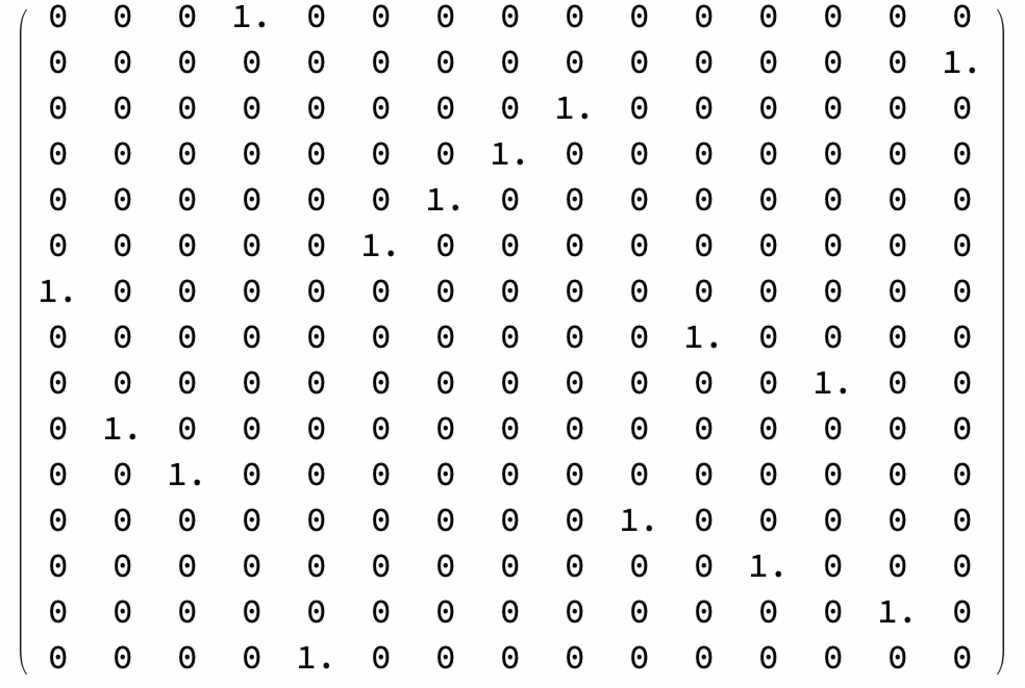
\includegraphics[width=1\textwidth]{PermR_LU.pdf}}\\
    \subfloat[Diagonal pivoting.]{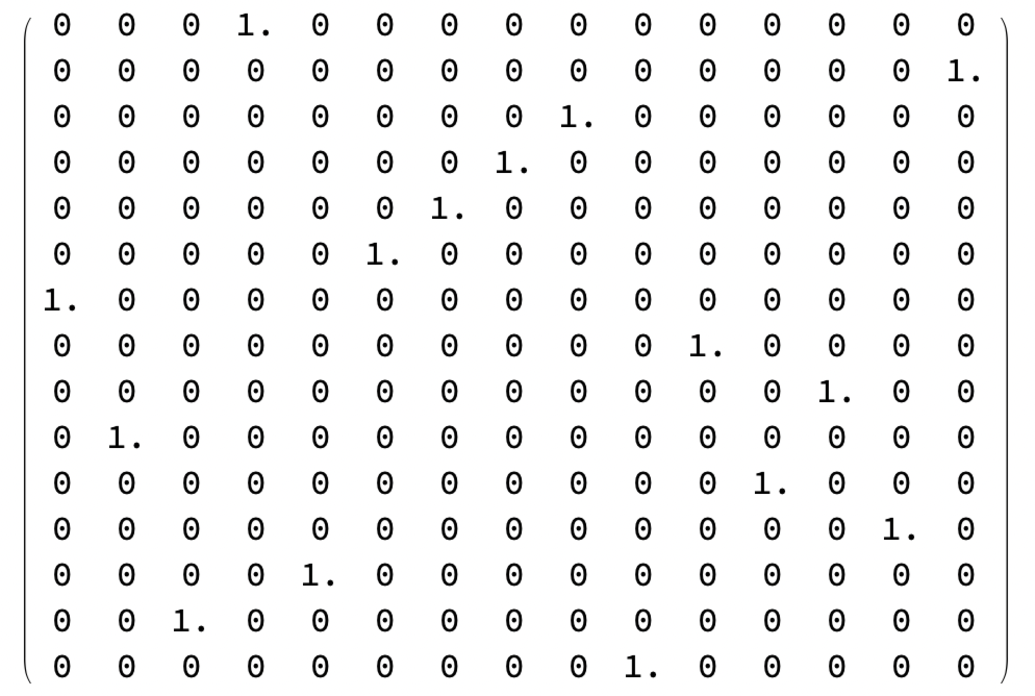
\includegraphics[width=1\textwidth]{PermR_LU_diag.pdf}}
    \caption{Row permutation matrix for LU decomposition.}
    \label{fig:PermutationMatrixRLU}
\end{figure}
\begin{figure}
    \centering
    \subfloat[Regular pivoting.]{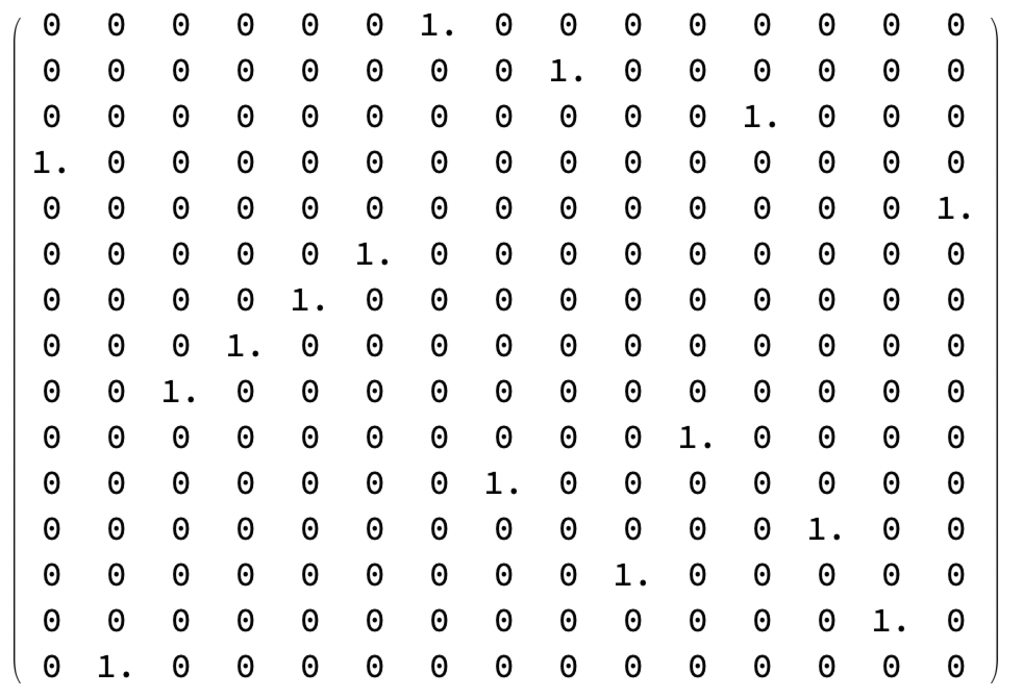
\includegraphics[width=1\textwidth]{PermC_LU.pdf}}\\
    \subfloat[Diagonal pivoting.]{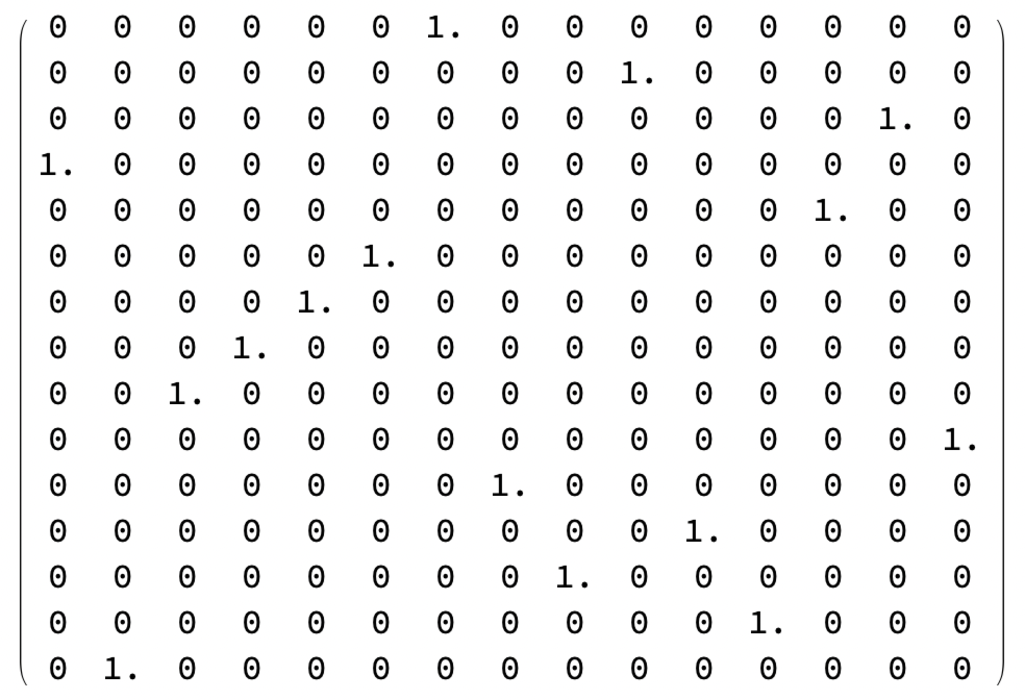
\includegraphics[width=1\textwidth]{PermC_LU_diag.pdf}}
    \caption{Columns permutation matrix for LU decomposition.}
    \label{fig:PermutationMatrixCLU}
\end{figure}

Figures \ref{fig:PermutationMatrixRLDLt} and \ref{fig:PermutationMatrixCLDLt} show the row and column permutation matrices for LDLt decomposition, respectively. Notice that due to the symmetry of the matrix, the column permutation matrix is the transpose of the row permutation matrix.
\begin{figure}
    \centering
    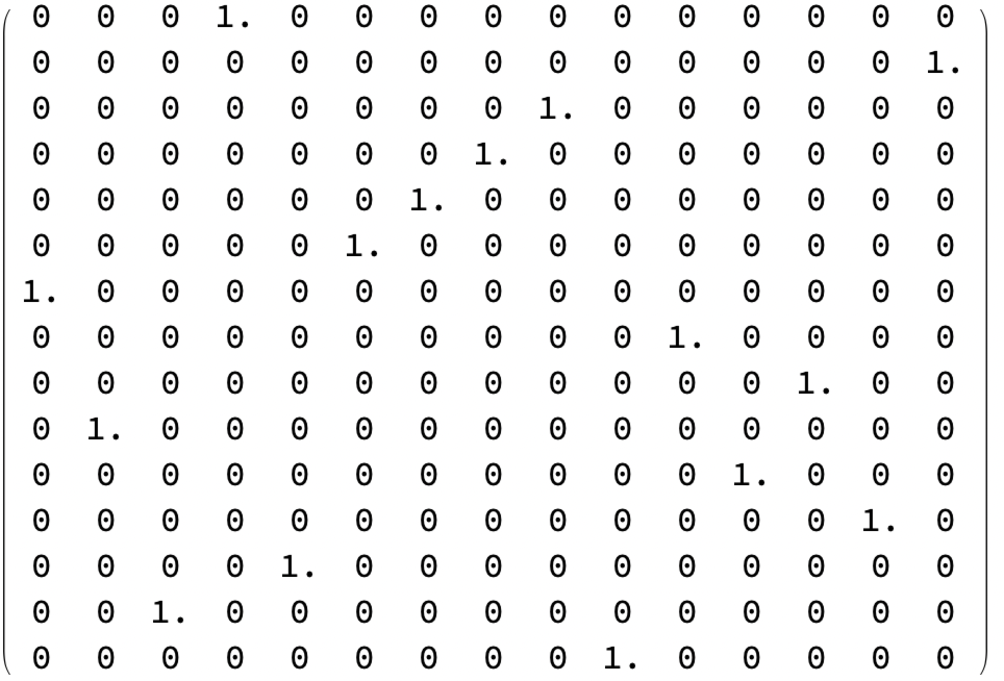
\includegraphics[width=1\textwidth]{PermR_LDLt.pdf}
    \caption{Row permutation matrix for LDLt decomposition.}
    \label{fig:PermutationMatrixRLDLt}
\end{figure}
\begin{figure}
    \centering
    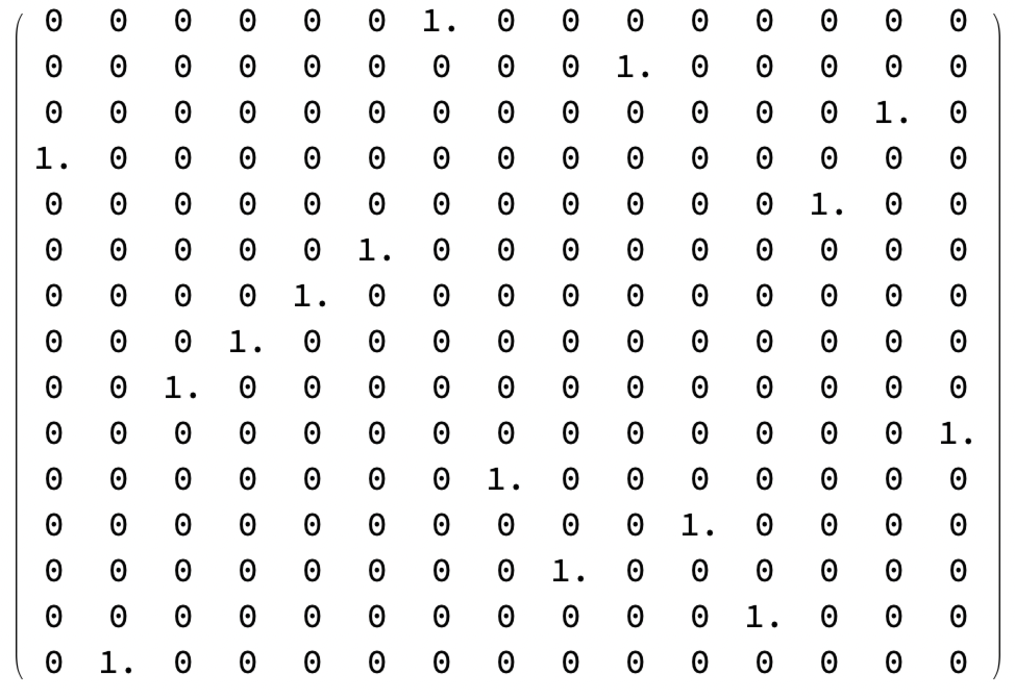
\includegraphics[width=1\textwidth]{PermC_LDLt.pdf}
    \caption{Columns permutation matrix for LDLt decomposition.}
    \label{fig:PermutationMatrixCLDLt}
\end{figure}